% A LaTeX template for EXECUTIVE SUMMARY of the MSc Thesis submissions to 
% Politecnico di Milano (PoliMi) - School of Industrial and Information Engineering
%
% S. Bonetti, A. Gruttadauria, G. Mescolini, A. Zingaro
% e-mail: template-tesi-ingind@polimi.it
%
% Last Revision: October 2021
%
% Copyright 2021 Politecnico di Milano, Italy. NC-BY

\documentclass[11pt,a4paper,twocolumn]{article}

%------------------------------------------------------------------------------
%	REQUIRED PACKAGES AND  CONFIGURATIONS
%------------------------------------------------------------------------------
% PACKAGES FOR TITLES
\usepackage{titlesec}
\usepackage{color}

% PACKAGES FOR LANGUAGE AND FONT
\usepackage[utf8]{inputenc}
\usepackage[english]{babel}
\usepackage[T1]{fontenc} % Font encoding

% PACKAGES FOR IMAGES
\usepackage{graphicx}
\graphicspath{{Images/}} % Path for images' folder
\usepackage{eso-pic} % For the background picture on the title page
\usepackage{subfig} % Numbered and caption subfigures using \subfloat
\usepackage{caption} % Coloured captions
\usepackage{transparent}

% STANDARD MATH PACKAGES
\usepackage{amsmath}
\usepackage{amsthm}
\usepackage{bm}
\usepackage[overload]{empheq}  % For braced-style systems of equations

% PACKAGES FOR TABLES
\usepackage{tabularx}
\usepackage{longtable} % tables that can span several pages
\usepackage{colortbl}

% PACKAGES FOR ALGORITHMS (PSEUDO-CODE)
\usepackage{algorithm}
\usepackage{algorithmic}

% PACKAGES FOR REFERENCES & BIBLIOGRAPHY
\usepackage[colorlinks=true,linkcolor=black,anchorcolor=black,citecolor=black,filecolor=black,menucolor=black,runcolor=black,urlcolor=black]{hyperref} % Adds clickable links at references
\usepackage{cleveref}
\usepackage[square, numbers, sort&compress]{natbib} % Square brackets, citing references with numbers, citations sorted by appearance in the text and compressed
\bibliographystyle{plain} % You may use a different style adapted to your field

% PACKAGES FOR THE APPENDIX
\usepackage{appendix}

% PACKAGES FOR ITEMIZE & ENUMERATES 
\usepackage{enumitem}

% OTHER PACKAGES
\usepackage{amsthm,thmtools,xcolor} % Coloured "Theorem"
\usepackage{comment} % Comment part of code
\usepackage{fancyhdr} % Fancy headers and footers
\usepackage{lipsum} % Insert dummy text
\usepackage{tcolorbox} % Create coloured boxes (e.g. the one for the key-words)
\usepackage{stfloats} % Correct position of the tables

%-------------------------------------------------------------------------
%	NEW COMMANDS DEFINED
%-------------------------------------------------------------------------
% EXAMPLES OF NEW COMMANDS -> here you see how to define new commands
\newcommand{\bea}{\begin{eqnarray}} % Shortcut for equation arrays
\newcommand{\eea}{\end{eqnarray}}
\newcommand{\e}[1]{\times 10^{#1}}  % Powers of 10 notation
\newcommand{\mathbbm}[1]{\text{\usefont{U}{bbm}{m}{n}#1}} % From mathbbm.sty
\newcommand{\pdev}[2]{\frac{\partial#1}{\partial#2}}
% NB: you can also override some existing commands with the keyword \renewcommand

%----------------------------------------------------------------------------
%	ADD YOUR PACKAGES (be careful of package interaction)
%----------------------------------------------------------------------------


%----------------------------------------------------------------------------
%	ADD YOUR DEFINITIONS AND COMMANDS (be careful of existing commands)
%----------------------------------------------------------------------------


% Do not change Configuration_files/config.tex file unless you really know what you are doing. 
% This file ends the configuration procedures (e.g. customizing commands, definition of new commands)
% Set the geometric layout of the document
\usepackage{geometry}
\geometry{
  top=3cm,
  left = 2.0cm,
  right = 2.0cm,
  bottom=2cm,
  headheight= 2cm,
  headsep= 0cm,
}
\raggedbottom 

% Create color bluePoli (-> manuale grafica coordinata:  https://www.polimi.it/fileadmin/user_upload/il_Politecnico/grafica-coordinata/2015_05_11_46xy_manuale_grafica_coordinata.pdf)
\definecolor{bluePoli}{cmyk}{0.4,0.1,0,0.4}

% Custom theorem environments
\declaretheoremstyle[
  headfont=\color{bluePoli}\normalfont\bfseries,
  bodyfont=\color{black}\normalfont\itshape,
]{colored}

\captionsetup[figure]{labelfont={color=bluePoli}} % Set colour of the captions
\captionsetup[table]{labelfont={color=bluePoli}} % Set colour of the captions
\captionsetup[algorithm]{labelfont={color=bluePoli}} % Set colour of the captions

\theoremstyle{colored}
\newtheorem{theorem}{Theorem}[section]
\newtheorem{proposition}{Proposition}[section]

% Enhances the features of the standard "table" and "tabular" environments.
\newcommand\T{\rule{0pt}{2.6ex}}
\newcommand\B{\rule[-1.2ex]{0pt}{0pt}}

% Algorithm description
\newcounter{algsubstate}
\renewcommand{\thealgsubstate}{\alph{algsubstate}}
\newenvironment{algsubstates}{
    \setcounter{algsubstate}{0}%
    \renewcommand{\STATE}{%
    \stepcounter{algsubstate}%
    \Statex {\small\thealgsubstate:}\space}
    }{}
    
% Custom theorem environment
\newcolumntype{L}[1]{>{\raggedright\let\newline\\\arraybackslash\hspace{0pt}}m{#1}}
\newcolumntype{C}[1]{>{\centering\let\newline\\\arraybackslash\hspace{0pt}}m{#1}}
\newcolumntype{R}[1]{>{\raggedleft\let\newline\\\arraybackslash\hspace{0pt}}m{#1}}

% Custom itemize environment
\setlist[itemize,1]{label=$\bullet$}
\setlist[itemize,2]{label=$\circ$}
\setlist[itemize,3]{label=$-$}
\setlist{nosep}

% Set separation of columns 
\setlength{\columnsep}{30pt}

% Create command for background pic
\newcommand\BackgroundPic{% Adding background picture
	\put(230,358){
		\parbox[b][\paperheight]{\paperwidth}{%
			\vfill
			\centering
			\transparent{0.4}
			
\includegraphics[width=0.5\paperwidth]{raggiera_polimi.eps}%
			\vfill
}}}

% Set indentation
\setlength\parindent{0pt}

% Custom title commands
\titleformat{\section}
{\color{bluePoli}\normalfont\Large\bfseries}
{\color{bluePoli}\thesection.}{1em}{}
\titlespacing*{\section}
{0pt}{2ex}{1ex}

\titleformat{\subsection}
{\color{bluePoli}\normalfont\large\bfseries}
{\color{bluePoli}\thesubsection.}{1em}{}
\titlespacing*{\subsection}
{0pt}{2ex}{1ex}

% Custom headers and footers
\pagestyle{fancy}
\fancyhf{}
      
\fancyfoot{}
\fancyfoot[C]{\thepage} % page
\renewcommand{\headrulewidth}{0mm} % headrule width
\renewcommand{\footrulewidth}{0mm} % footrule width

\makeatletter
\patchcmd{\headrule}{\hrule}{\color{black}\hrule}{}{} % headrule
\patchcmd{\footrule}{\hrule}{\color{black}\hrule}{}{} % footrule
\makeatother

% -> Create the header
\chead[C]{
\centering
\begin{tcolorbox}[arc=0pt, boxrule=0pt, colback=bluePoli!60, width=\textwidth, colupper=white]
    \textbf{} \hfill \textbf{\author}  
\end{tcolorbox}
}

% Insert here the info that will be displayed into your Title page 
% -> title of your work
\renewcommand{\title}{A review on chemical-kinetic models for hypersonic flows in thermochemical nonequilibrium}
% -> author name and surname
\renewcommand{\author}{Federico Cutolo}
% -> MSc course
\newcommand{\course}{Aeronautical Engineering}
% -> advisor name and surname
\newcommand{\advisor}{Prof. Giulio Gori}
% IF AND ONLY IF you need to modify the co-supervisors you also have to modify the file Configuration_files/title_page.tex (ONLY where it is marked)
%\newcommand{\firstcoadvisor}{Name Surname} % insert if any otherwise comment
%\newcommand{\secondcoadvisor}{Name Surname} % insert if any otherwise comment
% -> academic year
\newcommand{\YEAR}{2022-2023}

%-------------------------------------------------------------------------
%	BEGIN OF YOUR DOCUMENT
%-------------------------------------------------------------------------
\begin{document}

%-----------------------------------------------------------------------------
% TITLE PAGE
%-----------------------------------------------------------------------------
% Do not change Configuration_files/TitlePage.tex (Modify it IF AND ONLY IF you need to add or delete the Co-advisors)
% This file creates the Title Page of the document
% DO NOT REMOVE SPACES BETWEEN LINES!

\twocolumn[{\begin{@twocolumnfalse}

\AddToShipoutPicture*{\BackgroundPic}

\hspace{-0.6cm}
\includegraphics[width=0.6\textwidth]{logo_polimi_ing_indinf.eps}

\vspace{-1mm}
\fontsize{0.3cm}{0.5cm}\selectfont \bfseries \textsc{\color{bluePoli} In-depth analysis for the course Fundamentals of Hypersonic flows}\\

\vspace{-0.2cm}
\Large{\textbf{\color{bluePoli}{\title}}}\\

\vspace{-0.2cm}
\fontsize{0.3cm}{0.5cm}\selectfont \bfseries \textsc{\color{bluePoli} Laurea Magistrale in \course}\\

\vspace{-0.2cm}
\fontsize{0.3cm}{0.5cm} \selectfont \bfseries Author: \textsc{\textbf{\author}}\\

\vspace{-0.4cm}
\fontsize{0.3cm}{0.5cm}\selectfont \bfseries Person code: \textsc{\textbf{10521274}}\\

\vspace{-0.4cm}
\fontsize{0.3cm}{0.5cm}\selectfont \bfseries Advisor: \textsc{\textbf{\advisor}}\\

% if only ONE co-advisor is present:
%\vspace{-0.4cm}
%\fontsize{0.3cm}{0.5cm}\selectfont \bfseries Co-advisor: \textsc{\textbf{\firstcoadvisor}}\\
% if more than one co-advisors are present:
%\vspace{-0.4cm}
%\fontsize{0.3cm}{0.5cm}\selectfont \bfseries Co-advisors: \textsc{\textbf{\firstcoadvisor}}\textsc{\textbf{\secondcoadvisor}}\\

\vspace{-0.4cm}
\fontsize{0.3cm}{0.5cm}\selectfont \bfseries Academic year: \textsc{\textbf{\YEAR}}

\small \normalfont

\vspace{11pt}

\centerline{\rule{1.0\textwidth}{0.4pt}}

\vspace{15pt}
\end{@twocolumnfalse}}]

\thispagestyle{plain} % In order to not show the header in the first page

%%%%%%%%%%%%%%%%%%%%%%%%%%%%%%
%%     THESIS MAIN TEXT     %%
%%%%%%%%%%%%%%%%%%%%%%%%%%%%%%

%-----------------------------------------------------------------------------
% INTRODUCTION
%-----------------------------------------------------------------------------
\begin{abstract}
    The conservation equations for simulating hypersonic flows in thermal and chemical nonequilibrium for the Air-11 model are presented. The chemical-vibrational coupling is introduced with Park's two-temperature model, together with its reaction set and kinetic parameters. Park's model of 1987 is compared with the models of Park 1991, Gupta, Dunn-Kang. The comparison is based on a numerical study of the heat flux on the surface of the Apollo command module at $Ma=20.5$. The differences between the models are ascribed to the difference in reaction rates involving $N_2$ and $O_2$.
\end{abstract}

\section{Introduction}
\label{sec:introduction}

Re-entry vehicles in hypersonic high enthalpy re-entry flows encounter thermochemical nonequilibrium states (Fig.\ref{fig:nonequilibrium}). Nonequilibrium processes occur in a flow when the time required for a process to accommodate itself to local conditions within some region is of the same order as the transit time across that region. If the accommodation time is very short compared with the transit time, the process is in equilibrium. If the accommodation time is very long compared with the transit time, the process is frozen. The length scale of the region depends on what is being studied. A useful length scale could be the shock stand-off distance. The ongoing process can be a chemical reaction or an exchange in energy between energy degrees of freedom (translational, rotational,  vibrational, electronic). 

In the Air-11 model, the accommodation process takes place with collisions of heavy particles (molecules, atoms, ions) among themselves or with electrons. The accommodation time is given by the frequency of the collisions. Even though the collision rate might be high enough to keep the velocity distribution functions close to the equilibrium (Maxwellians), the number of effective collisions, in terms of vibrational energy transfer or chemical reaction, might be much smaller. In this case, the vibrational or chemical relaxation is not fast enough to keep the local thermochemical equilibrium. Hence, it is necessary to model vibrational and chemical kinetics in a coupled fashion to prescribe accurate chemical rate coefficients and, ultimately, attain a precise description of the heat flux around the body.


%-----------------------------------------------------------------------------
% EQUATIONS AND FIGURES
%-----------------------------------------------------------------------------
\section{Conservation Equations}
\label{sec:equations}
High-temperature air is assumed to be composed of the following 11 species: $N_2$, $O_2$, $N$, $O$, $NO$, $N_2^+$, $O_2^+$, $NO^+$, $N^+$, $O^+$, $e^-$. The conservation equations for a reacting gas flow in which thermal nonequilibrium is modeled with a three-temperature approximation ( i.e., three-energy equations ) can be expressed as follows.\\

\textit{Species conservation}:
\begin{equation}\label{eq:species}
      \frac{\partial \rho_s}{\partial t}+\frac{\partial \rho_s u^j}{\partial x^j}=\frac{\partial}{\partial x^j}(\rho D_s\frac{\partial y_s}{\partial x^j})+\dot w_s
\end{equation}
\textit{Mixture Momentum conservation}:
\begin{multline}\label{eq:momentum}
    \frac{\partial}{\partial t}\rho u^i+\frac{\partial}{\partial x^j}\rho u^i u^j=-\frac{\partial p}{\partial x^i} \hfill\\+\frac{\partial}{\partial x^j}\left [ \mu \left(\frac{\partial u^i}{\partial x^j}+\frac{\partial u^j}{\partial x^i}\right)-\frac{2}{3}\mu\frac{\partial u^k}{\partial x^k} \delta^{ij}\right ] \hfill
\end{multline}
The pressure $p$ is defined as
\begin{equation}
    p = \sum_{s=1}^{11}p_s
\end{equation}
and the partial pressure of species $s$ is defined by
\begin{equation}
    p_s = \frac{\rho_s\bar R T}{M_s}
\end{equation}
Where $M_s$ is the molecular weight of species $s$, and $\bar R$ is the universal gas constant. $\mu$ is the mixture viscosity.\\ 

\textit{Vibrational Energy conservation}
\begin{multline}\label{eq:vibrational}
     \frac{\partial}{\partial t}\rho e_v+\frac{\partial}{\partial x^j}\rho e_v u^j = \frac{\partial}{\partial x^j}\left( \eta_v \frac{\partial T_v}{\partial x^j}\right)\\+\frac{\partial}{\partial x^j}\left(\rho\sum_{s=1}^{11} h_{e,s}D_s\frac{\partial y_s}{\partial x_j} \right)+ \dot Q_{v-t} \hfill\\+ \dot Q_{v-e} +\sum_{s=1}^{N_{mol}}\dot w_s \hat{D_s}\hfill
\end{multline}
Were the vibrational energy per unit mass $e_v$ is defined as:
\begin{equation*}
    e_v = \sum_{s=1}^{11}\frac{\rho_s e_{v,s}(T_e)}{\rho}
\end{equation*}
The second term of the right-hand side is the conduction of vibrational energy across the control volume due to vibrational temperature gradients. The third term of the right-hand side represents the diffusion of vibrational energy due to concentration gradients. $\dot Q_{v-t}$ and $\dot Q_{v-e}$ are the rate of energy exchange between vibrational and translational modes and between vibrational and electronic modes due to collisions within the volume, respectively:
\begin{align*}
     \dot Q_{v-t}=\sum_{s=1}^{N_{mol}}\rho_s\frac{(e_{v,s}^*-e_{v,s})}{<\tau_s>}\\
     \dot Q_{v-e}=\sum_{s=1}^{N_{mol}}\rho_s\frac{(e_{v,s}^{**}-e_{v,s})}{<\tau_{es}>} 
\end{align*}
Where $e_{v,s}^*$ and $e_{v,s}^{**}$ are the vibrational energy of species $s$ evaluated at the roto-translational temperature and electronic temperature respectively, while $e_{v,s}$ is the total vibrational energy associated with the species. 
The last term accounts for the vibrational energy loss or gain due to chemical reactions of dissociation and recombination respectively. $\hat{D}_s$ is the vibrational energy per unit mass of the diatomic molecules, created or destroyed at a rate $\dot w_s$.\\

\textit{Electron and Electron Excitation Energy conservation}:
\begin{multline}\label{eq:electronic}
    \frac{\partial}{\partial t}\rho e_e + \frac{\partial}{\partial x^j}\left[ u^j(\rho e_e + p_e)\right] = u^j\frac{\partial p_e}{\partial x^j}\hfill\\+\frac{\partial}{\partial x^j}\left(\eta_e \frac{\partial T_e}{\partial x^j}\right) + \frac{\partial}{\partial x^j}\left(\rho\sum_{s=1}^{11}h_{e,s}D_s\frac{\partial y_s}{\partial x^j} \right)\hfill\\+\dot C_{h-e}(T_e) + \dot Q_{v-e} - \dot I^e -\dot Q_{rad}\hfill
\end{multline}\\
Where the terms of the left-hand side represent the rate of change of electronic energy per unit volume in a cell-centered at $x^j$ and the flux of electronic enthalpy across cell walls with velocity $u^j$. In particular\\
\begin{equation*}
e_e = \sum_{s=1}^{11}\frac{\rho_s e_{e,s}(T_e)}{\rho}
\end{equation*}
The first term on the right-hand side represents the work done by electrons subject to electron pressure gradients. $\dot C_{h-e}(T_e)$ is the energy exchange due to collision between heavy particles and electrons. $\dot Q_{v-e}$ is again the rate of energy exchange between electronic and vibrational modes. $\dot I^e$ embeds the energy loss due to ionization of molecules and atoms, where electrons are lost. $\dot Q_{rad}$ represents the rate of energy loss due to radiation, where electrons transit from upper to lower energetic levels.\\

\textit{Total Energy conservation}
\begin{multline}\label{eq:total}
    \frac{\partial}{\partial t}\rho E + \frac{\partial}{\partial x^j} \rho H u^j =\hfill\\ \frac{\partial}{\partial x^j} \left(\eta\frac{\partial T}{\partial x^j}+\eta_v\frac{\partial T_v}{\partial x^j}+ \eta_e\frac{\partial T_e}{\partial x^j}\right) \hfill\\ +\frac{\partial}{\partial x^j}\left( \rho\sum_{s=1}^{11} h_s D_s \frac{\partial y_s}{\partial x^j} \right)+\dot S + \dot Q_{rad}\hfill
\end{multline}

The total energy is defined as
\begin{equation*}
    E = \frac{1}{2}u^iu^i + \sum_{s=1}^{11}\frac{\rho_s e_s}{\rho}
\end{equation*}
while the total enthalpy is defined as
\begin{equation*}
    H = E + \frac{p}{\rho}
\end{equation*}
$\dot S$ represents the work done by shear forces.
The conservation equations were taken from \cite{lee1984basic}. 

\section{Two-temperatures model}
The three-temperatures model used to define the equations \ref{eq:species}-\ref{eq:total} considers the partitioning of energy among the modes can be described by three temperatures $T$, $T_v$ and $T_e$, which are the roto-translational\footnote{The hypothesis behind the coupling of rotational and translational equilibrium is that they have a similar relaxation time, and small compared to the vibrational and electronic ones.}, vibrational and electronic temperatures respectively. What constitutes an adequate description of the energy distribution is subjective. For the purpose of simulating flow fields around hypersonic vehicles, an \textit{adequate} model is the one that allows an accurate prediction of convective and radiative heating of the surface. More detailed models tried to describe the vibrational energy of each species with a different vibrational temperature. Multivibrational temperature models accuracy relies on the availability of experimental data related to the species relaxation time, and so constitute a far more complicated way, and yet not-so-adequate to describe the roto-translational temperature \cite{gnoffo1989conservation}. 

Park presented in 1987 a two-temperature model based on the observed \cite{park1988assessment}:
\begin{itemize}
    \item fast energy exchange between translational modes of free electrons and the vibrational mode of $N_2$;
    \item fast equilibration of the lower electronic states of heavy particles (molecules, atoms, ions) at the temperature associated with the ground electronic state.
\end{itemize}
In the 2-T model, the translational and rotational energies are treated as one equilibrium energy mode specified by a roto-translational temperature $T_{rt}$. The electron translation, electronic excitation, and species vibrational energies are treated as one nonequilibrium energy mode represented by the electron-electronic-vibrational temperature $T_{ev}$. The 2-T model is obtained by combining equations \ref{eq:vibrational} and \ref{eq:electronic} in one.\\

\textit{Vibrational-Electronic Energy conservation}
\begin{multline}\label{eq:vibratioal-electronic}
     \frac{\partial}{\partial t}\rho e_{ev}+\frac{\partial}{\partial x^j}\rho e_{ev} u^j = -p_e\frac{\partial u^j}{\partial x^j}\hfill \\+\frac{\partial}{\partial x^j}\left[ (\eta_v+ \eta_e) \frac{\partial T_{ev}}{\partial x^j}\right]\hfill\\ +\frac{\partial}{\partial x^j}\left(\rho\sum_{s=1}^{11} h_{ev,s}D_s\frac{\partial y_s}{\partial x_j} \right) +\dot Q_{v-t}\hfill \\+\dot C_{h-e}(T_{ev})-\dot I^e + \sum_{s=1}^{N_{mol}}\dot w_s \hat{D_s}+ \dot Q_{rad} \hfill
\end{multline}
Where the vibrational-electronic energy (property of the mixture) and vibrational-electronic enthalpy for species $s$ per unit mass are :
\begin{align*}
    e_{ev} = & e_v + e_e\\
    h_{ev,s} = & h_{v,s}+h_{e,s}
\end{align*}
\section{Chemical-kinetic models}
The mass rate production of species $s$ per unit volume appearing in \ref{eq:vibratioal-electronic} and \ref{eq:vibrational} is expressed as \cite{gnoffo1989conservation, sarma2000physico}
\begin{multline}
    \dot w_s = M_s \sum_{r=1}^{N_r}\left( \beta_{s,r}-\alpha_{s,r}\right)\cdot\\\left[ k_{f,r}\prod_{s=1}^{11}\left(\frac{\rho_s}{M_s}\right)^{\alpha_{s,r}}\hfill- k_{b,r}\prod_{s=1}^{11}\left(\frac{\rho_s}{M_s}\right)^{\beta_{s,r}}\right]\hfill
\end{multline}\\
Where $N_r$ is the total number of reactions taking place, $\alpha_{s,r}$ and $\beta_{s,r}$ are the stoichiometric coefficients for reactants and products in the $r$ reaction respectively. $k_{f,r}$ and $k_{b,r}$ are the forward and backward coefficients for the reaction $r$ respectively.
\subsection{Chemical-vibrational coupling}
In the literature, two types of chemical-vibrational coupling have been proposed: preferential and non-preferential dissociation. The first claims that dissociation of molecular species is obtained more easily when they are vibrationally excited. Despite so, when the conditions are highly energetic (very high velocities) the dissociation may occur at lower levels, in a non-preferential way. The present work is devoted to comparing four preferential chemical-vibrational couplings models: Park-87, Park-91, Gupta and Dunn-Kang.
\subsection{Reaction rates}
The forward rate coefficients of the chemical reaction for all four models is obtained by the Arrhenius formula \cite{blottner1969viscous}
\begin{equation}\label{eq:arrhenius}
    k_{f,r}=C_{f,r}T^{n_{f,r}}_d exp\left( \frac{-E_{f,r}}{k T_d}\right)
\end{equation}
Where $C_{f,r}$, $n_{f,r}$ and the activation energy $E_{f,r}$ divided by the Boltzmann constant $k$ are kinetic parameters established empirically for a set of chemical reactions involving the eleven species of air. The temperature $T_d$ is a dummy variable for the rate-controlling temperature, and in all four cases is assumed to be the geometric average of the roto-translational and the vibrational temperatures. The temperature is heavily weighted by the vibrational temperature, because of the preferential concept, in the following way:
\begin{equation}
    T_d = \sqrt{TT_{v}}
\end{equation}

Park-87 and Park-91 models prescribe a backward rate coefficient that depends on the equilibrium constant of the reaction $K_r$
\begin{equation}
    k_{b,r}=\frac{k_{f,r}(T)}{K_{r}}
\end{equation}
The equilibrium constants of Park-87 and Park-91 models are evaluated by the following curve fits of temperature, respectively:
\begin{align*}
    \ln(K_{r}) = &A + B \ln(Z) + C Z + D Z^2 + E Z^3\\
    \ln(K_{r}) = &A/Z + B + C \ln(Z) + D Z + E Z^2
\end{align*}
Where $Z=10^4/T$, and coefficients A, B, C, D, E are parameters of each chemical reaction available in  \cite{park1988assessment, park1991chemical} respectively. The backward rate coefficients in Dunn-Kang model are obtained by Arrhenius form \cite{dunn1973theoretical}
\begin{equation}
    k_{b,r}=C_{b,r}T^{n_{b,r}}_d exp\left( \frac{-E_{b,r}}{k T_d}\right)
\end{equation}
For velocities below $8$ $km/s$, the backward rate coefficients of Gupta model are evaluated by Arrhenius formula \ref{eq:arrhenius}. For higher velocities, the backward rate coefficients of Gupta model are obtained from the equilibrium constants \cite{gupta1990review}:
\begin{equation}
      k_{b,r}= \frac{k_{f,r}(T_d)}{K_{r}(T_d)} 
\end{equation}
Generally speaking, the chemical-kinetic models are defined by a set of elementary reactions, equilibrium constants and relative parameters for each reaction, forward and backward coefficients formulations, and the rate-controlling temperature. All four models presented share the same rate-controlling temperature and the same form of the forward rate coefficient. They hence differ in the set of elementary equations among the eleven species, relative parameters to define the equilibrium constant in addition to the backward rate coefficient formulation. 
\section{Comparison}
A comparative study by Wang \cite{wang2017assessment} of the the four kinetic models is now presented and commented. The comparison was carried out numerically with a in-house code developed by Wang et al. in \cite{wang2016laminar}. The test-case studied is the Apollo command module, a typical geometry for re-entry vehicles. The Apollo typical flow features are visible in Fig.\ref{fig:apollo}. The free stream conditions, which are taken from the AS-202 flight test \cite{walpot2012base}, are listed in Tab.\ref{tab:freestream}.

\begin{figure}[h]
    \centering
    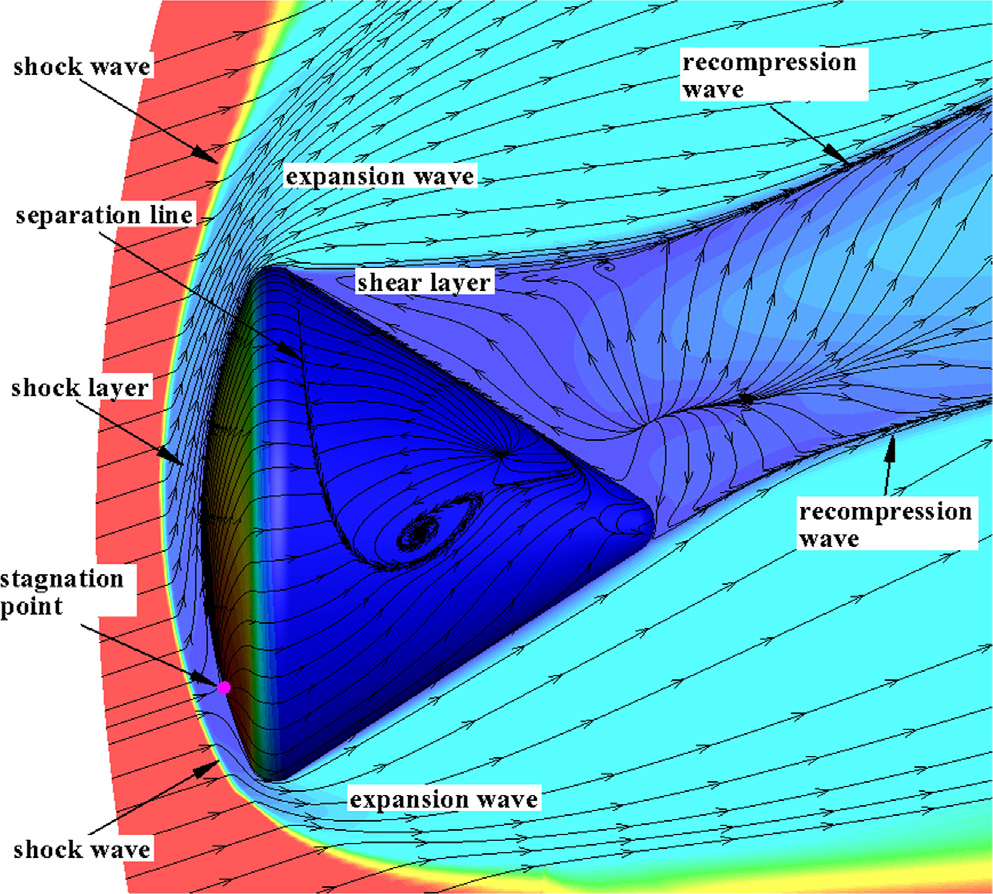
\includegraphics[width=0.47\textwidth]{myimages/apollo flow features.png}
    \caption{Apollo capsule flow features}
    \label{fig:apollo}
\end{figure}

\begin{table}[h]
    \centering
    \begin{tabular}{|c|c|c|c|}
    \hline
    \hline
        $U$ (m/s) &  $Ma$ & AoA (deg)& H (km)\\
        \hline
       6210 & 20.5 & 18.4 & 67.3\\   
       \hline
       \hline
    \end{tabular}
    \caption{Freestream conditions}
    \label{tab:freestream}
\end{table}

The grid used features 1.86 million cells, and it is visible in Fig.\ref{fig:grid}. The heat flux is evaluated for the four kinetic models and plotted around the symmetry plane in Fig.\ref{fig:comparison}.

\begin{figure}[h]
    \centering
    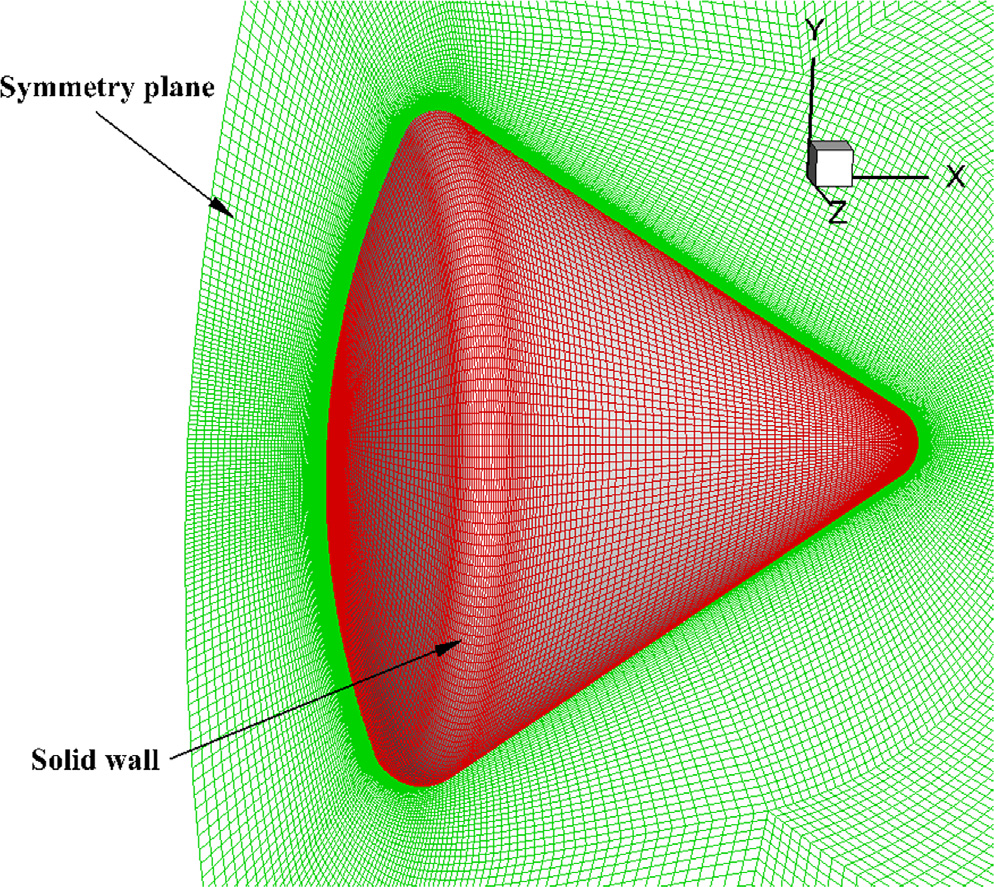
\includegraphics[width=0.47\textwidth]{myimages/grid.png}
    \caption{Grid. Windside and leeside corners are refined to capture the expansions}
    \label{fig:grid}
\end{figure}

\begin{figure}
    \centering
    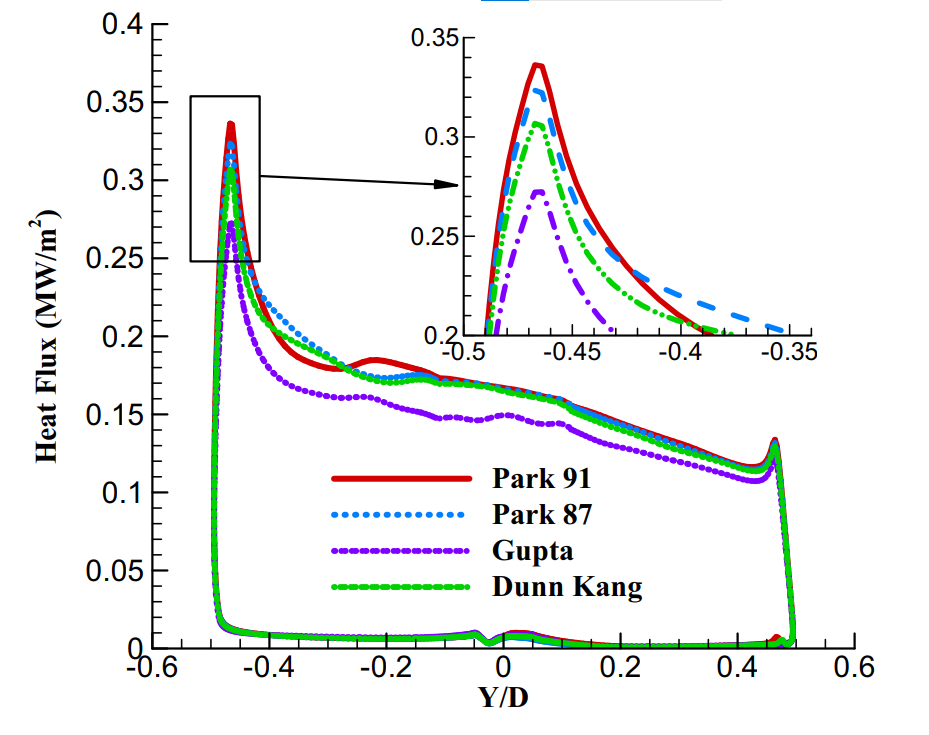
\includegraphics[width=0.47\textwidth]{myimages/comparison.png}
    \caption{Heat flux profile around the symmetry plane cut}
    \label{fig:comparison}
\end{figure}

The heat flux at the forebody of the vehicle predicted by Gupta model is lower than the results computed with the other three models, whose heat flux shows similar behaviour. In the most part of the forebody the heat fluxes predicted by Dunn-Kang model, Park-87 model and Park-91 model are nearly the same, which are about $20\%$ higher than Gupta model. At the backbody of the vehicle, the aeroheating environment predicted by the four chemical kinetic models do not show any significant difference. The peak of heat flux is observed for all models at the same location, at the windside shoulder of the body, and are reported in Tab\ref{tab:heatflux}. The maximum difference is about $27\%$. 

\begin{table}[h]
    \centering
    \begin{tabular}{|c|c|c|c|c|}
    \hline
    \hline
                            & P-87 & P-91 & D-K & Gupta \\
                            \hline
     $\dot q$ ($MW/m^2$)    & 0.305 &  0.270  & 0.325 & 0.335  \\
     \hline
     \hline
    \end{tabular}
    \caption{Peak values of the heat flux for the four models}
    \label{tab:heatflux}
\end{table}

Numerical heat flux prediction along the Apollo’s surface exhibits a relatively strong sensitivity to the choice of chemical kinetic models. This difference appears to be increasing for increasing complexity of the vehicle geometry and increasing Mach number\cite{wang2017assessment}. To investigate the reason for these discrepancies, the chemical rates of dissociation and recombination of molecular nitrogen and molecular oxygen are compared for the four chemical-kinetic models.
\begin{align*}
        & N_2+N_2\rightleftharpoons 2N+N_2\\
        & O_2+O_2\rightleftharpoons 2O+O_2
\end{align*}

If for the dissociation of $N_2$ there's no substantial difference (Fig.\ref{fig:n2dissociation}), a sensible difference for the Gupta model is appreciated in the dissociation rate of $O_2$ along the whole temperature span (Fig.\ref{fig:o2dissociation}). Furthermore, conspicuous differences are noticed in the recombination rates of both molecular species (Fig.\ref{fig:n2recombination},\ref{fig:o2recombination}). 

\begin{figure}[h]
    \centering
    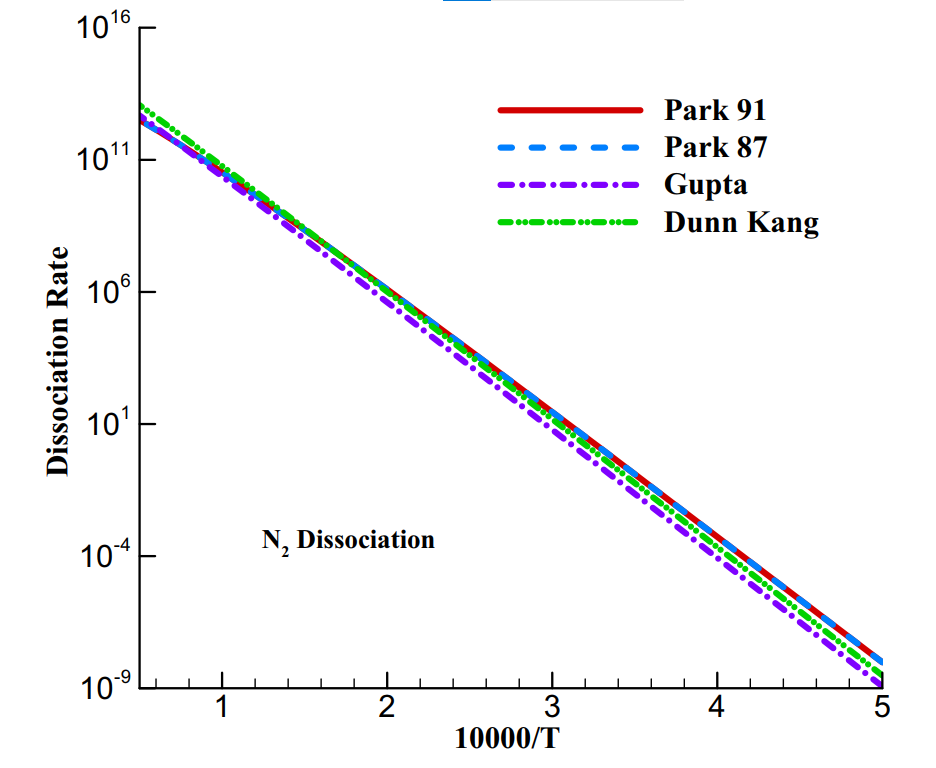
\includegraphics[width=0.47\textwidth]{myimages/N2dissociation.png}
    \caption{Dissociation rate of $N_2$ as function of rate temperature $T_d$}
    \label{fig:n2dissociation}
\end{figure}

\begin{figure}[h]
    \centering
    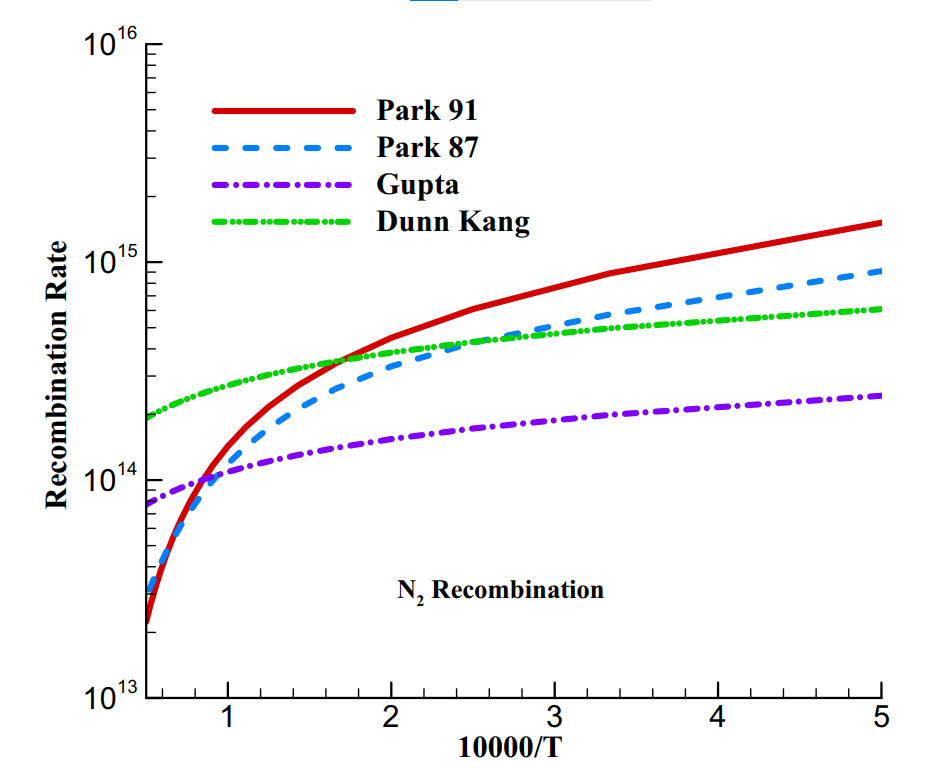
\includegraphics[width=0.47\textwidth]{myimages/N2recombination.png}
    \caption{Recombination rate of $N_2$ as function of $T_d$}
    \label{fig:n2recombination}
\end{figure}

\begin{figure}[h]
    \centering
    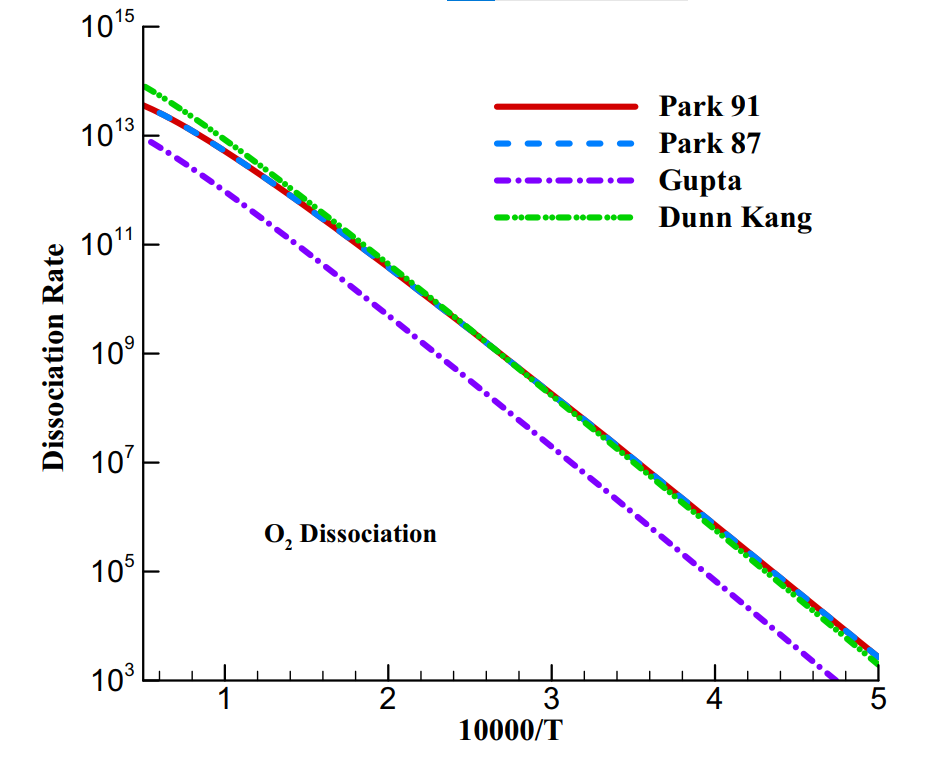
\includegraphics[width=0.47\textwidth]{myimages/O2dissociation.png}
    \caption{Dissociation rate of $O_2$ as function of rate temperature $T_d$}
    \label{fig:o2dissociation}
\end{figure}

\begin{figure}[h]
    \centering
    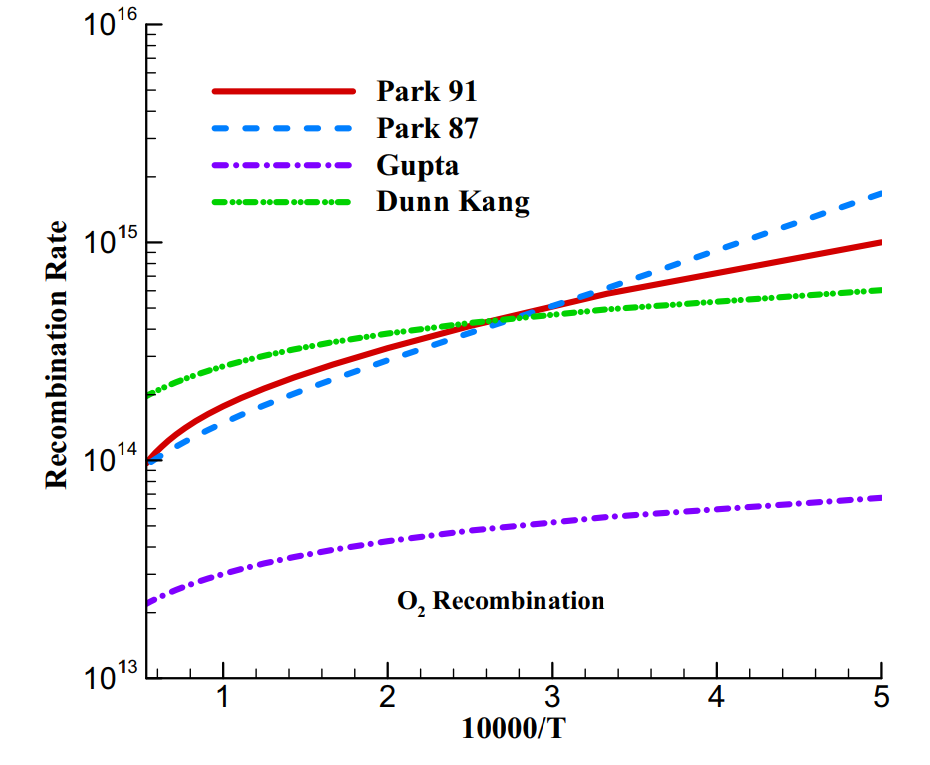
\includegraphics[width=0.47\textwidth]{myimages/O2recombination.png}
    \caption{Recombination rate of $O_2$ as function of $T_d$}
    \label{fig:o2recombination}
\end{figure}

In the same work, Wang et al. \cite{wang2017assessment} show, for a different test case, the influence of the choice of a chemical-kinetic model on the shock standoff distance. Also, Gnoffo et al. \cite{gnoffo1989conservation} noticed the standoff distance of the Park-87 and Dunn-Kang models was slightly different. However, due to the lack of enough flight data and a poor understanding of the chemical kinetic mechanism, it is difficult to judge which chemical kinetic model is better, and large uncertainties still exist in the chemical kinetic models. 
%-----------------------------------------------------------------------------
% CONCLUSION
%-----------------------------------------------------------------------------
\section{Concluding remarks}
The conservation equations for simulating hypersonic flows in thermal and chemical nonequilibrium are presented for the three-temperature model. The two-temperature model is obtained by joining the Vibrational and Electron-Electronic Energy conservation equations. Therefore, Park's two-temperatures model of 1987 is introduced and compared with its modification of 1991, the Gupta model and the Dunn-Kang model, in terms of reaction rates. To assess the differences, the test case of Apollo module re-entry at $Ma=20.5$ is considered. The heat flux at the forebody surface is noticed to be substantially affected by the choice of the chemical-kinetic model. The reason for these differences in the heat flux peaks of the four models is attributed by Wang \cite{wang2017assessment} to the difference in the reaction rates for the dissociation and recombination of molecular nitrogen and molecular oxygen. Nevertheless, Gnoffo \cite{gnoffo1989conservation} and Hao \cite{hao2016numerical} claim that the major impact of the choice of a kinetic model is ascribed to the ionization reactions. \\
In general, there is still no concrete evidence to indicate which chemical reaction model can predict better results than the other, for the simulation of hypersonic reentry flowfields. Given the lack of enough validation data and a deeper understanding of the physical mechanism of chemical kinetic models, the validity of these models is difficult to assess and large differences and uncertainties still exist in their definition.
\section{Final notes}
\subsection{The limits of updating empirical models}
Recent works on the determination of dissociation and recombination rate coefficients \cite{kim2021modification}\cite{helber2017determination}\cite{panerai2012characterization} still hinge on modified versions of legacy models, as Park and Dunn-Kang models, based on better experimental data and computations. These updated models stand on the same basis as the legacy ones, dragging with them the poor understanding of the physical inference of those chemical-kinetic models.
\subsection{Future outlook}
Nowadays, the scientific community is moving towards predictive models to control natural phenomena. In this framework, model calibration acquires a critical role in its validation. The incomplete understanding of the physical implication of a model makes its uncertainty unknown and its calibration inaccurate, ultimately leading to results with unknown reliability outside the competence of the specific experimental case. That is why it is of essential importance that uncertainty assessment is led during the construction of the empirical model, starting from the assumptions about the experimental data and post-processing \cite{del2021bayesian}\cite{del2023stochastic}.

%------------------------------------------------------
%  BIBLIOGRAPHY
%---------------------------------------------------------------------------
% Remember to insert here only the essential bibliography of your work
\bibliography{bibliography.bib} % automatically inserted and ordered with this command 
\onecolumn
\appendix
\begin{figure}[]
    \centering
    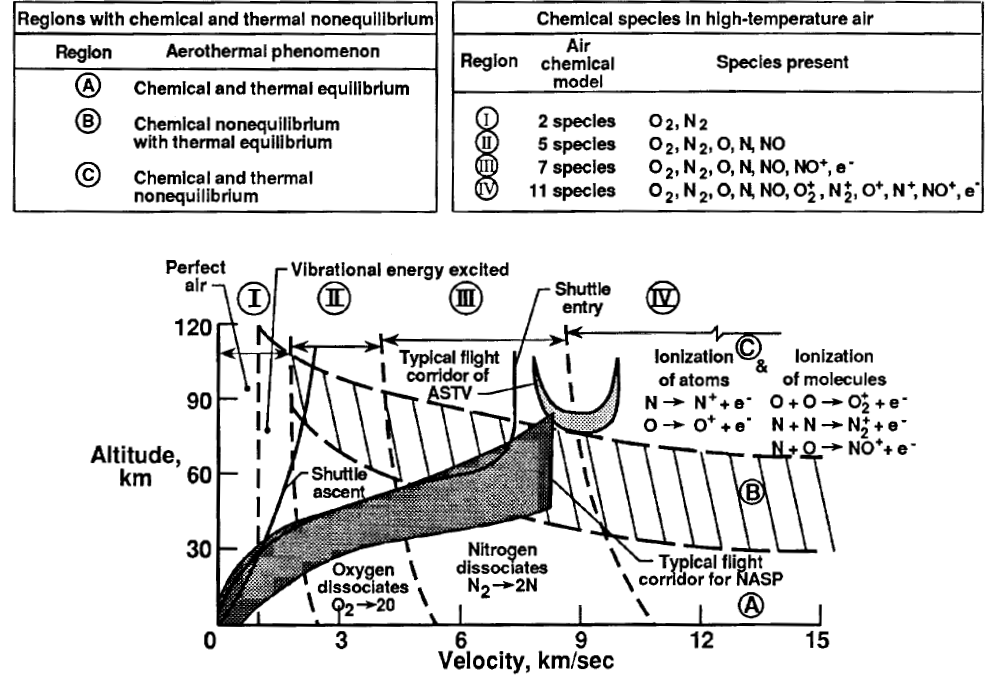
\includegraphics[width=1\textwidth]{myimages/regimes.png}
    \caption{Chemistry of the stagnation region for a sphere of $30.5$ cm radius (taken from Hansen \cite{hansen1958review})}
    \label{fig:nonequilibrium}
\end{figure}
\end{document}